\section{Webcamsteuerung}
\Diskussionspunkt{evtl. gehört das Thema Webcam ins Kapitel Sensoren}
Zur Wetterstation Arbon gehört auch eine Webcam der Marke Axis. Diese ist auch wieder über ein Applikationsplugin in die Webseite integriert. Auf dieser können per Shortlinks sechs verschiedene Positionen angefahren werden.

\begin{figure}[h]
	\centering
	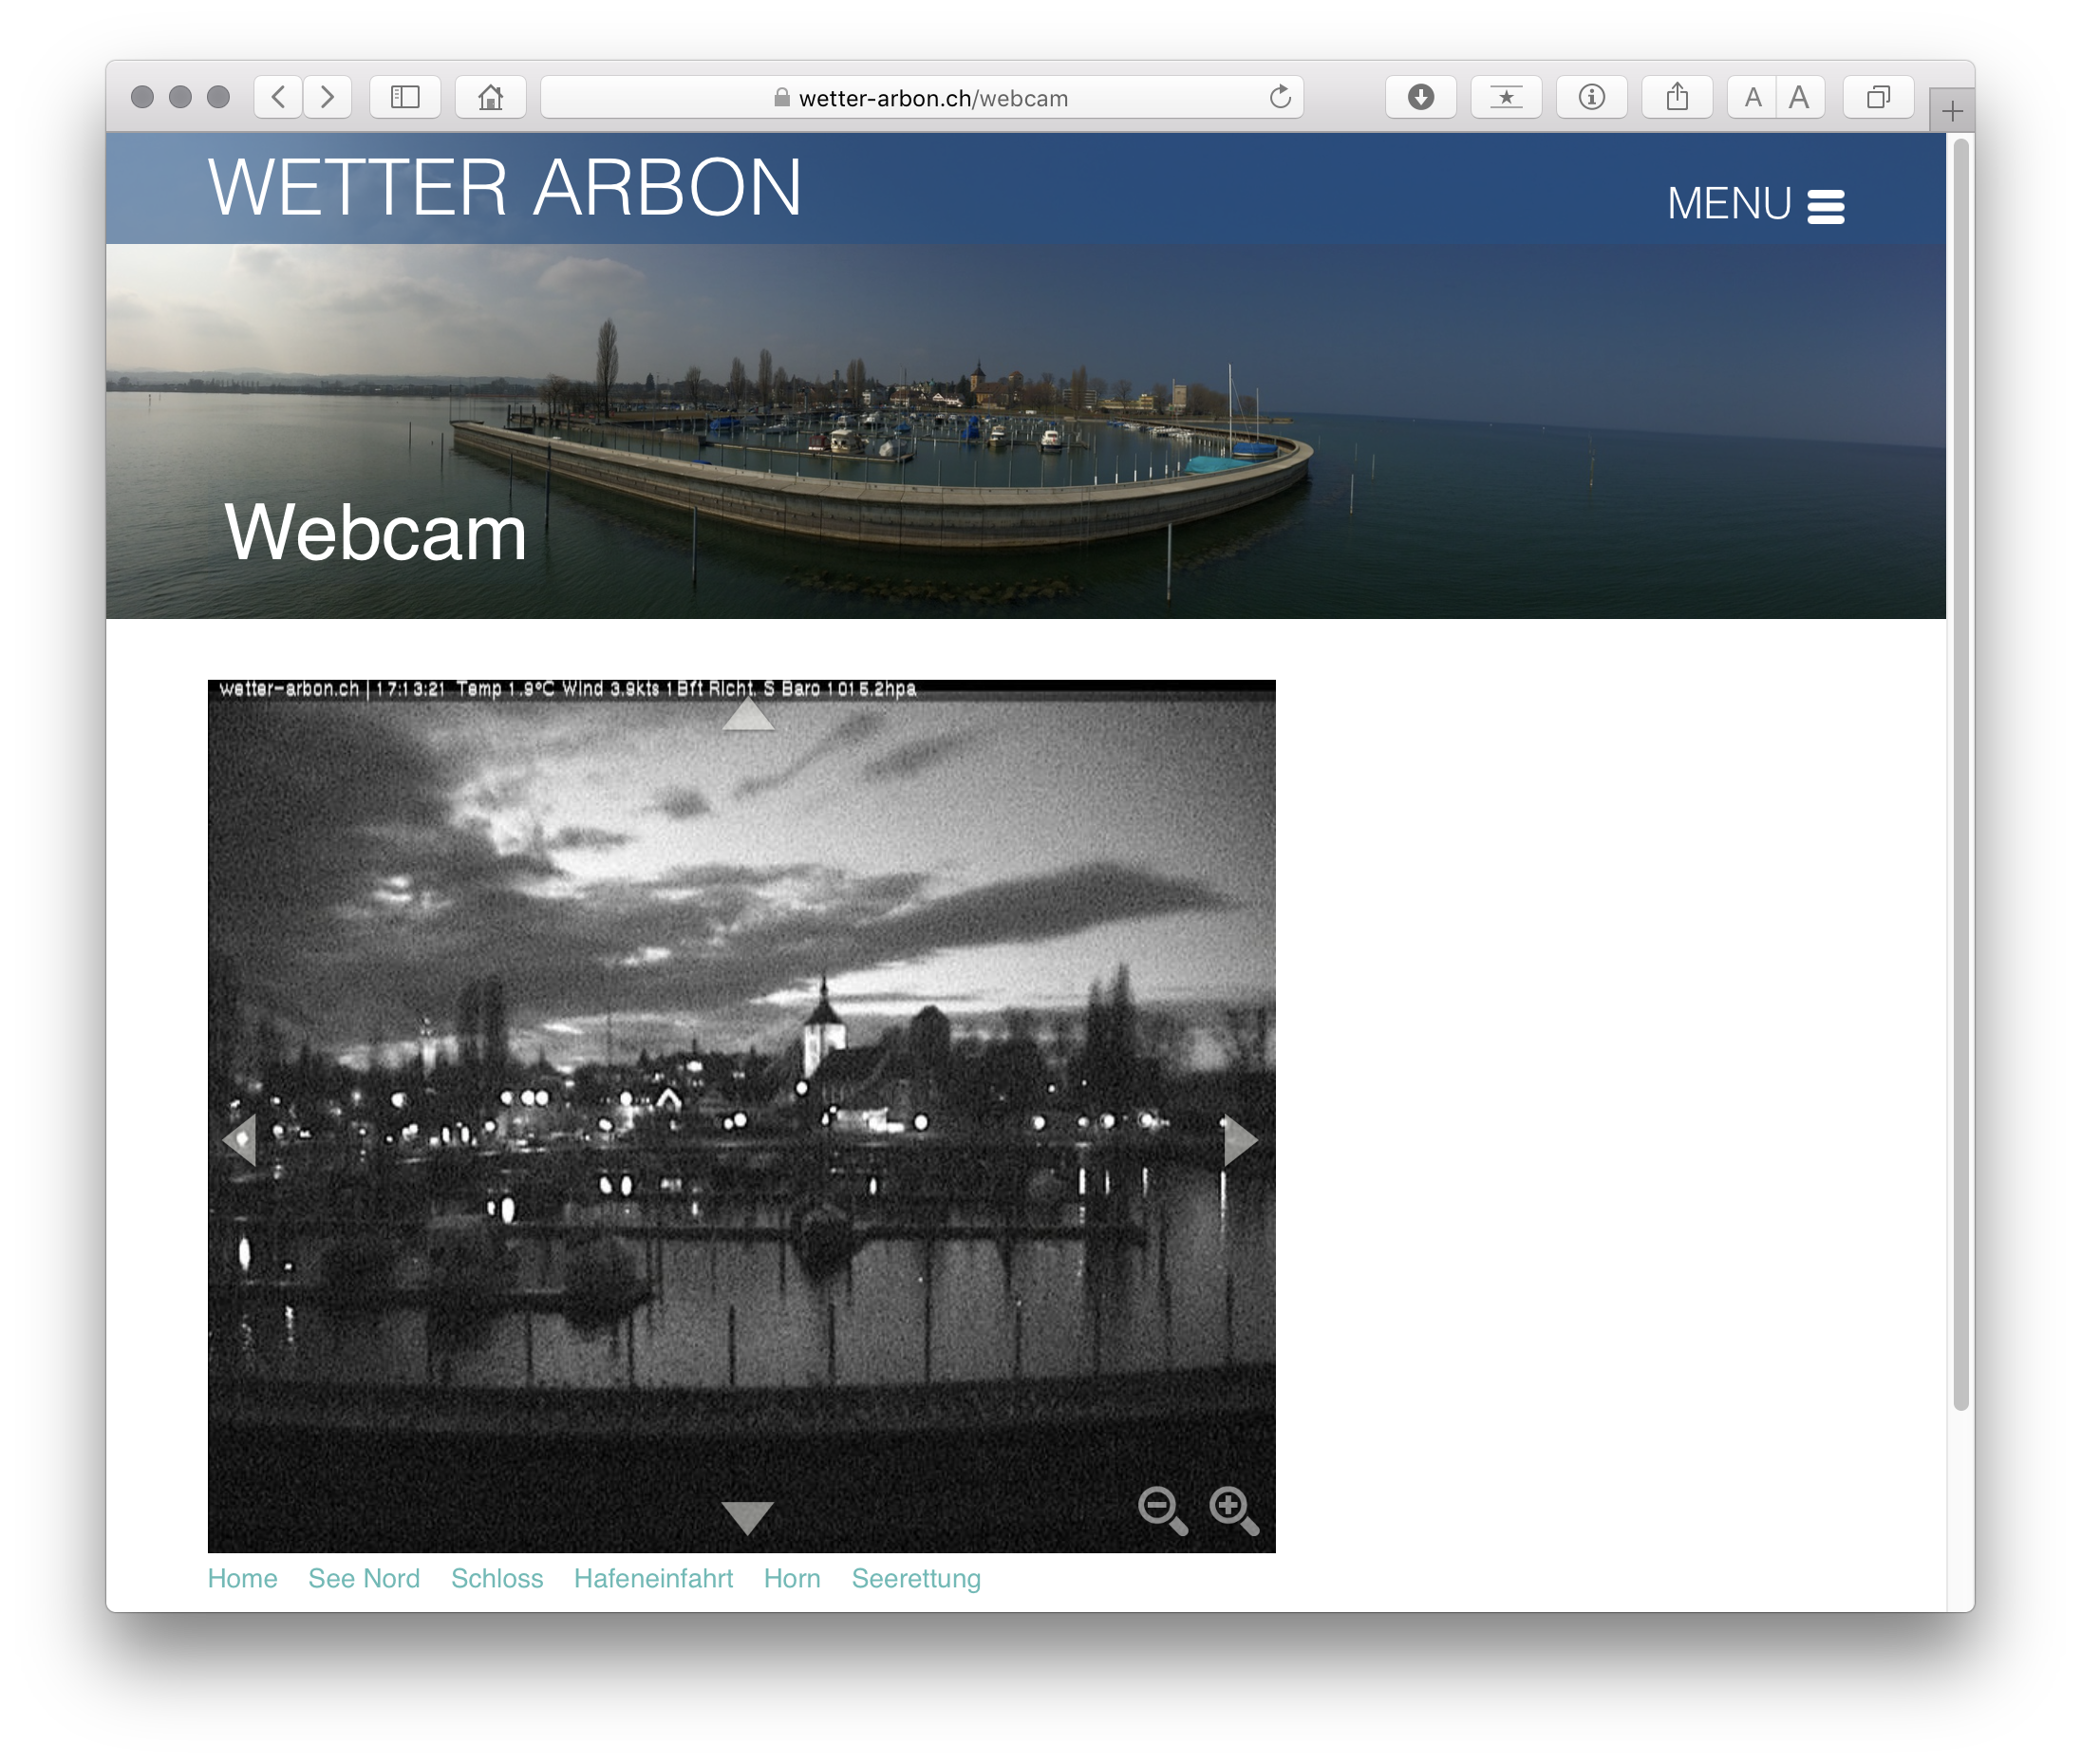
\includegraphics[width=1\linewidth]{img/webcam-seite}
	\caption{Ansicht und Steuerung der Webcam}
	\label{img:webcam-seite}
\end{figure}


% Positionierung / Abfrage der Position
\subsection{Positionsbestimmung}
Diese Positionen sind in der Betriebseigenen Software konfiguriert. Neben den voreingestellten Positionen, kann die Kamera auch frei Positioniert werden. Diese freie Positionierung erfolgt über Pfeile, sowie die Plus und Minus am Bildrand, je nachdem welcher Button geklickt wird, sendet die Webseite das Kommando mittels HTTP an die Webcam. Die Zusammenstellung der URL geschieht über ein Javascript, wie man dem folgenden Code entnehmen kann.


\begin{lstlisting}[caption={Webcam},label={lst:cam},language=html]
 <div class="container webcam" id="webcam_585">
	<img class="pageImage" src="https://webcam.wetter-arbon.ch/mjpg/video.mjpg" alt="" />
</div>
<script type="text/javascript">
	function changeWebCam(command) {
		var urlAddition;
		switch (command) {
			case 'up':
			case 'down':
			case 'left':
			case 'right':
			case 'home':
				urlAddition = 'move=' + command;
				break;
				
			case 'zoomIn':
				urlAddition = 'rzoom=2500';
				break;
				
			case 'zoomOut':
				urlAddition = 'rzoom=-2500';
				break;
				
			case 'Hafeneinfahrt':
				urlAddition = 'gotoserverpresetname=' + command;
				break;		
		}
		console.log('changeWebCam');
		$.get('https://webcam.wetter-arbon.ch/axis-cgi/com/ptz.cgi?camera=1&' + urlAddition);
	}
\end{lstlisting}


% Zoom
\subsection{Selektive Zoombeschränkung}
In der Betriebseigenen Software lassen sich viele Parameter Konfigurieren, wie auch der Zoomfaktor. Diese ist jedoch aus Datenschutzgründen auf die 4-fache Vergrösserung limitiert, möglich wäre aber eine 216-fache Vergrösserung. Daraus wird schon deutlich das die Webcam mehr Potential hat und die Limitierung des Zooms in der BA so Konfiguriert werden, dass diese möglichst dynamisch sein. D.h., dass jenach Position der Zoomfaktor auch mit ändert. Der Zoom soll, vor allem auf den See hinaus in vollem Umfang benutzt werden können. Die Position der Kamera kann mit einer einfachen HTTP GET anfrage aufgerufen werden. Daraus wird ersichtlich in welche Richtung die Kamera zeigt und kann so, mittels einem einfachen Javascript den Zoom beschränken oder erweitern.

% Warteschlange
\subsection{Warteschlange}
\Diskussionspunkt{Problem ohne Warteschlange, mögliche Implementierung}


